\documentclass[12pt,a4paper,twoside,onecolumn,titlepage]{report}
\usepackage[utf8]{inputenc}
\usepackage[T1]{fontenc}
\usepackage{todonotes}
\usepackage{url}
\usepackage[english,polish]{babel}
\usepackage{cite}
\usepackage{listings}
\usepackage{xcolor}
\usepackage{floatrow}
\usepackage[section]{placeins}
\floatsetup[table]{capposition=top}
\colorlet{punct}{red!60!black}
\definecolor{background}{HTML}{EEEEEE}
\definecolor{delim}{RGB}{20,105,176}
\colorlet{numb}{magenta!60!black}
\definecolor{javared}{rgb}{0.6,0,0} % for strings
\definecolor{javagreen}{rgb}{0.25,0.5,0.35} % comments
\definecolor{javapurple}{rgb}{0.5,0,0.35} % keywords
\definecolor{gray}{rgb}{0.4,0.4,0.4}
\definecolor{darkblue}{rgb}{0.0,0.0,0.6}
\definecolor{cyan}{rgb}{0.0,0.6,0.6}
\lstdefinelanguage{json}{
	basicstyle=\normalfont\ttfamily,
	numbers=left,
	numberstyle=\scriptsize,
	stepnumber=1,
	numbersep=8pt,
	showstringspaces=false,
	breaklines=true,
	frame=lines,
	backgroundcolor=\color{background},
	literate=
	*{0}{{{\color{numb}0}}}{1}
	{1}{{{\color{numb}1}}}{1}
	{2}{{{\color{numb}2}}}{1}
	{3}{{{\color{numb}3}}}{1}
	{4}{{{\color{numb}4}}}{1}
	{5}{{{\color{numb}5}}}{1}
	{6}{{{\color{numb}6}}}{1}
	{7}{{{\color{numb}7}}}{1}
	{8}{{{\color{numb}8}}}{1}
	{9}{{{\color{numb}9}}}{1}
	{:}{{{\color{punct}{:}}}}{1}
	{,}{{{\color{punct}{,}}}}{1}
	{\{}{{{\color{delim}{\{}}}}{1}
	{\}}{{{\color{delim}{\}}}}}{1}
	{[}{{{\color{delim}{[}}}}{1}
	{]}{{{\color{delim}{]}}}}{1},
}

\lstset{
	showstringspaces=false,
	frame=single,
	breaklines=true,
	numbers=left,
	basicstyle=\ttfamily,
	keywordstyle=\color{javapurple}\bfseries,
	stringstyle=\color{javared},
	commentstyle=\color{javagreen},
}

\lstdefinelanguage{XML}
{
	morestring=[b]",
	morestring=[s]{>}{<},
	morecomment=[s]{<?}{?>},
	stringstyle=\color{black},
	identifierstyle=\color{darkblue},
	keywordstyle=\color{cyan},
	morekeywords={xmlns,version,type}% list your attributes here
}
\begin{document}
\begin{otherlanguage}{english} 
\begin{abstract}
\begin{center}
\textbf{Comparative analysis of Apache Hadoop and Apache Spark solutions for big data parallel processing.}\newline
\end{center}
The topic of this thesis is touching relatively new information technology domain which is Big Data. This master thesis is focusing mainly on two most popular open source platforms used in Big Data processing: Apache Spark and Apache Hadoop. The most crucial part of thesis is comprehensive comparison of both platforms in such manner that end user can estimate, which tool is faster, cheaper in further development and maintenance. Additionally, this master thesis is attempting to answer question, whether it is cost effective to migrate from Apache Hadoop to Apache Spark and vice-versa. During research web application was developed in order to obtain throughput results for comparative analysis and further development easyness. Big Data source has been \textit{Twitter Developer API} which allows to use service public data updated in real time. Application was based on two programming languages: Scala and Java, used \textit{Play!} framework and application lifecycle management tool \textit{Scala Build Tool}. Source code management was realized via \textit{Git}.         
\end{abstract}
\end{otherlanguage}
\begin{otherlanguage}{polish} 
\begin{abstract}
\begin{center}
\textbf{Analiza porównawcza rozwiązań Apache Hadoop i Apache Spark dedykowanych równoległemu przetwarzaniu danych masowych.}
\end{center}
Tematyka niniejszej pracy magisterskiej dotyczy niedawno powstałej dziedziny informatyki, jaką jest przetwarzanie danych masowych. Praca magisterska skupia się głównie na dwóch najpopularniejszych narzędziach używanych w procesie przetwarzania danych masowych dostępnych na licencji otwartego kodu źródłowego: Apache Spark i Apache Hadoop. Najważniejszym elementem pracy jest kompleksowe porównanie obu platform tak, by dać użytkownikowi możliwość oceny, które narzędzie jest szybsze, tańsze w rozwijaniu i utrzymaniu oraz czy warto migrować z jednej platformy na drugą i odwrotnie. Podczas przeprowadzonych badań powstała aplikacja internetowa, która posłużyła jako narzędzie dostarczające wyniki wydajności dla analizy porównawczej, jak również łatwości pod względem dalszego rozwoju. Źródłem danych masowych jest \textit{Twitter Developer API}, które udostępnia publiczne dane serwisu aktualizowane w czasie rzeczywistym. Aplikacja została opracowana w dwóch językach programowania Scala oraz Java, jednocześnie wykorzystuje ramę projektową \textit{Play!} oraz narzędzie do budowania i zarządzania cyklem dostarczania oprogramowania \textit{Scala Build Tool}. Wersjonowanie kodu źródłowego zostało zrealizowane przy pomocy systemu kontroli wersji \textit{Git}. 
\end{abstract}
\end{otherlanguage}
\tableofcontents
\chapter{Wstęp} \label{chap.introduction}
{placeholder}

\section{Problematyka operacji w kontekście platform równoległych. Batch, streaming, operacje leniwe.}
W dzisiejszym świecie występują ogromne ilości danych, które są produkowane przez człowieka. Daje to ogromne możliwości do wszelkiego rodzaju wnioskowań, aczkolwiek jednocześnie wymaga ogromnego nakładu pracy. W związku w upowszechnieniem się automatyzacji zaczęto pracować nad koncepcją przetwarzania danych w sposób równoległy tak aby proces przebiegał jak najszybciej i efektywniej. Takie podejście do przetwarzania danych zrodziło problemy, które musiały zostać rozwiązane aby zyski ze skomplikowania architektury obliczeń przewyższyły koszty. Jednym z największych wyzwań podczas zrównoleglenia obliczeń jest synchronizacja danych zależnych jak również ich poprawność w danej jednostce czasu w danej części systemu obliczeń. Jednocześnie dzięki takiemu podejściu zaoszczędzono nakład pracy poświęcony na konstruowanie komputera o dużej mocy obliczeniowej, który byłby w stanie wykonywać zadania sekwencyjnie zachowując takie same wyniki jeżeli chodzi o szybkość obliczeń. Komputery o dedykowanej architekturze procesora zastąpiono sprzętem dedykowanym dla przeciętego użytkownika, które w połączeniu dwóch lub więcej utworzyły klaster. Taka architektura pozwala na oszczędności w krótko oraz długo terminowym okresie czasu. Cena zakupu wielu komputerów, jest zazwyczaj niższa niż jeden komputer o dużej mocy obliczeniowej, utrzymanie jest również tańsze gdyż nie jest wymagana kadra o wąskiej specjalizacji. Dodatkowym aspektem może być również system chłodzenia - dedykowany dla komputera o dużej mocy. Standardowy komputer posiada wbudowany system chłodzenia, który nie wymaga uwzględnienia w kosztorysie. W kontekście przetwarzania równoległego przy rozważaniu danych masowych możemy rozróżnić dwa rodzaje przetwarzania: \textbf{batch} oraz \textbf{streaming}.
\subsection{Batch}\label{batch_subsection} 
Batch jest pojęciem zdefiniowanym w tym samym czasie gdy pojawiły się same komputery. Jest to wykonywanie poszczególnych operacji bez nadzoru człowieka (interaktywności). W kontekście danych masowych możemy przyjąć, że są to operacje analizy danych, które nie są wykonywane w czasie rzeczywistym np. generacja raportu na podstawie danych, które zostały zebrane od wielu klientów sklepu. Człowiek definiuje zadanie, programuje proces obliczeń, podaje dane wejściowe i oczekuje na wyniki dostarczone przez system informatyczny. Takie działanie charakteryzuje się odczuwalnym czasem oczekiwania (nie mylić z latencją). Jednocześnie użytkownik nie koniecznie potrzebuje wyników obliczeń natychmiastowo. Takie podejście może satysfakcjonować końcowego użytkownika, jeżeli chodzi o koszty obliczeń w zestawieniu do czasu otrzymania rezultatów.
\subsection{Streaming}\label{streaming_subsection}
Streaming (przetwarzanie strumieniowe) - jest pojęciem antagonistycznym do przetwarzania typu batch, jednocześnie w swojej implementacji wykorzystuje jego założenia. Streaming to przetwarzanie danych w czasie rzeczywistym - dostarczenie wyników dla użytkownika bez zauważalnego czasu czasu oczekiwania. Takie podejście jest często wykorzystywane podczas notowań giełdowych gdzie wartości indeksów spółek zmieniają się bardzo szybko w krótkiej ilości czasu. Jednocześnie użytkownik oczekuje rezultatów obliczeń jak najszybciej, by decyzja jakie akcje sprzedać/kupić mogła zostać podjęta. Streaming to przetwarzanie danych, które napływają w sposób ciągły, są dystrybuowane na mniejsze części (batch) i delegowane do obliczeń. Po uzyskaniu rezultat jest zwracany do użytkownika. W takim podejściu użytkownik jest nakierowany na krótki czas oczekiwania i błyskawiczną informację zwrotną. Moc obliczeniową sprzętu dedykuje się pod dane wejściowe tak by osiągnąć jak najkrótszy czas odpowiedzi a latencję (czas obsługi żądania obliczeń po stronie serwera wykonującego obliczenia) stara się minimalizować do poziomu zera.
\subsection{Operacje leniwe}
Operacje leniwe to technika stosowana by zoptymalizować obliczenia. Polega na opóźnianiu obliczeń do momentu aż rezultat nie jest faktycznie wymagany. Można przyjąć, że "potokuje" poszczególne operacje jednocześnie unikając zbędnej wymiany danych. Prostym przykładem może być zapisanie odczyt dużego pliku danych, zliczeniu wystąpień zadanej frazy i zapisanie wyniku w postaci innego pliku. Jeżeli taką akcję zdefiniujemy jako leniwą całe obliczenie zostanie wywołane w momencie zapisania do pliku wynikowego. Jeżeli zapisanie do pliku wynikowego nie zostanie uruchomione operacje odczytu pliku, filtrowania po zadanej frazie również. Dzięki temu obciążenie systemu obliczeń nie jest generowane do momentu, aż jest to faktycznie potrzebne. 

\section{Cele pracy}
Głównym celem pracy jest dogłębna analiza dwóch narzędzi do przetwarzania danych masowych w architekturze równoległej: Apache Spark\footnote{\url{http://spark.apache.org/}} oraz Apache Hadoop.\footnote{\url{https://hadoop.apache.org/}} Spark to projekt dosyć nowy projekt o otwartym kodzie źródłowym. Pierwsze wydanie nastąpiło 30 maja 2014. Wersja poddana badaniom to 2.1.0 wydana 28 grudnia 2016. Hadoop to narzędzie już dobrze znane na rynku ETL\footnote{Extract,Transform,Load} (pierwsze wydanie 27 grudnia 2001), wersja poddana analizie to 2.7.3 wydana 25 sierpnia 2016. Hadoop to rozwiązanie również na licencji otwartego kodu źródłowego. Analiza dotyczy takich czynników jak:
\begin{itemize}
	\item Wymagania sprzętowe, które stawiają oba narzędzia, które muszą być spełnione aby dostarczyć rezultaty obliczeń
	\item Wyniki czasowe przetwarzania zadanej próbki wejściowej
	\item Złożoność obsługi obu platform
	\item Koszty rekrutacji oraz szkolenia kadry wyspecjalizowanej w danej platformie
\end{itemize}
Do analizy powstało narzędzie oparte na szkielecie aplikacji internetowych Play\footnote{\url{https://playframework.com/}}, które udostępnia interfejs HTTP dla operacji przetwarzania danych dla obydwu platform. Narzędzie to posłużyło do dostarczenia rezultatów, które mogły zostać poddane analizie ze względu na kryteria podane powyżej. Poza badaniami wykonanymi w pracy dokonana została ocena możliwości komercyjnego rozwoju prototypowego narzędzia powstałego na potrzeby analizy. Dodatkowo oceniona została opłacalność migracji z narzędzia Apache Hadoop na Apache Spark ze względu na wymagania końcowego użytkownika. 

\section{Przegląd literatury}
\todo{Czy ten rozdział jest potrzebny?}
\section{Przegląd rozdziałów}
\todo{krótkie opisy poszczególnych rozdziałów}
\chapter{Przetwarzanie danych masowych na platformach\\równoległych} \label{chap.big-data-processing}

\section{Podstawowe definicje}
\subsection{Big data}
Definicja pojęcia Big data (dane masowe) jest dosyć rozległa i jednocześnie rozmyta. Świat informatyki kieruje się ku definicji iż big data występuje wszędzie tam gdzie wymagane jest przetworzenie wielkiej ilości danych. Jednocześnie nie jest zdefiniowana jednostka oraz jej wielkość od której możemy mówić o big data. Firma SAS opisuje termin big data jako: \newline \textit{"Big data is 
a  popular  term  used  to  describe  the  exponential  growth,  
availability  and  use  of  information,  both  structured  and  
unstructured"}. \newline Z kolei firma IBM big data definiuje jako: \textit{“Data, 
coming  from  everywhere;  sensors  used  to  gather  climate  
information,  posts  to  social  media  sites,  digital  pictures  
and  videos,  purchase  transaction  record,  and  cell  phone  
GPS signal to name a few”}.\cite{big_data_concept} Bazując na powyższym źródle możemy stwierdzić iż big data to zwyżkujący trend, który wskazuje na błyskawiczny przyrost danych pochodzących z różnych źródeł w krótkim okresie czasu. Jednocześnie wskazujący na znaczącą wartość danych po ich późniejszym przetworzeniu. Dla końcowego użytkownika, można uprościć, że big data to niedefiniowany zbiór różnych danych zawierający wartościowe informacje w nieuporządkowanej formie.
\subsection{4V}
W związku z mocno niedoprecyzowanym pojęciem big data publikacje naukowe definiują wymiary, które określają właściwości danych masowych.\cite{big_data_great_services} Kategorie te określa się pojęciem \textbf{4V}. Jest to skrót opisujący cztery wartości:
\begin{itemize}
	\item Objętość (Volume)
	\item Różnorodność (Variety)
	\item Prędkość (Velocity)
	\item Wiarygodność (Veracity)
\end{itemize}
Objętość wynika z samego rozmiaru danych. W założeniach są to rozmiary wielkie lecz nie można zdefiniować dokładnej wielkości oraz jednostki od której można stwierdzić iż dany zbiór danych już się kwalifikuje do zbioru big data. Brak jasno określonej wielkości ma sens ze względu na założenie, że zbiór big data jest nieskończony i stale rosnący. W związku z czym wielkość wymiaru ulega ciągłej zmianie.\newline
Różnorodność zakłada dane o nie jednorodnej strukturze. Użytkownik działający w środowisku big data jest nastawiony na dużą ilość danych, jednocześnie jest przygotowany na zorganizowanie ich samodzielnie w logiczną strukturę danych. Różnorodność to również wiele formatów danych: tekst, multimedia, grafika, dźwięk.\newline
Prędkość mówi o tempie generacji danych, które są tworzone przez wiele różnych podmiotów: ludzi, maszyn, wszelkiego rodzaju czujników. Jest to również pośrednie do samej techniki przetwarzania danych \textbf{streaming} \ref{streaming_subsection}.\newline
Wiarygodność to nic innego jak stopień poprawności danych. Wiele danych może być wygenerowanych błędnie, mogą być niekompletne, uszkodzone. Użytkownik systemu danych masowych musi samemu zdefiniować stopień do którego ufa danym na podstawie których dokonuje analizy.\newline
Ostatnim wymiarem, który nie podlega bezpośrednio terminowi 4V jest wartość (value). Jest to nie jako wypadkowa tego terminu - jaką wartość końcową stanowią dla użytkownika końcowego dane masowe. Czy wynik ich analizy przynosi realną wartość, czy koszty poniesione w stosunku do pozyskania oraz przetworzenia danych były niższe niż warość uzyskanych rezultatów?
\subsection{Klaster komputerowy}
Klaster komputerowy to najbardziej podstawowa jednostka obliczeniowa jeżeli chodzi o systemy rozproszone. Jest to zestaw połączonych między sobą samodzielnych komputerów, które mogą wymieniać wzajemnie informacji. Połączenie komputerowe opiera się o łącze o wysokiej przepustowości np. Ethernet, co gwarantuje obniżenie kosztów dystrybucji danych. Każda maszyna włączona do klastra posiada własny procesor obliczeniowy, pamięć RAM\footnote{Random access memory}, przestrzeń dyskową. Jednocześnie z punktu widzenia końcowego użytkownika, klaster posiada jeden punkt wejściowy dla obliczeń (API)\footnote{Application programmer interface}. Dzięki temu końcowy użytkownik nie jest zmuszony do zarządzania zasobami wewnętrznymi klastra i obsługuje tylko jedno źródło wprowadzania danych.\cite{cluster_grid_cloud} 
\newline Główną zaletą klastrów obliczeniowych jest wysoka dostępność. Z racji swojej rozproszonej architektury, która udostępnia łatwą skalowalność wszerz, możliwe jest dokładanie kolejnych komputerów by zwiększyć moc obliczeniową. Jednocześnie gdy moc obliczeniowa w danej jednostce czasu nie jest wymagana, komputery mogą zostać dynamicznie oddelegowane w stan uśpienia lub do innych zadań. Takie rozwiązanie jest bardzo elastyczne ze względu na potrzeby końcowego użytkownika. Dodatkowym aspektem jest stabilność klastrów. Gdy jakiś z elementów klastra ulega awarii, system monitoringu może łatwo wyszukać wadliwą jednostkę, usunąć ją z klastra i dołożyć nową, sprawną. Takie działanie pozwala użytkownikowi na korzystaniu z bardzo stabilnego rozwiązania, bez konieczności redukcji mocy obliczeniowej.\cite{cluster_grid_cloud_detailed_comparison}
\subsection{Obliczenia równoległe}
Obliczenia równoległe to rozdzielanie poszczególnych zadań dla niezależnych procesów, które z definicji posiadają osobną przestrzeń pamięci. Takie podejście jest wykorzystywane podczas przetwarzania danych masowych w klastrze komputerowym (każda maszyna jest oddzielnym procesem). Dzięki temu większość operacji jest wykonywana niezależnie co pozwala na zaoszczędzenie czasu w stosunku do obliczeń wielowątkowych, które zakładają zależność między sobą. Prof. Charles E. Leiserson wykładający na uczelni MIT\footnote{Massachusetts Institute of Technology} definuje obliczenia równoległe jako:
\newline \textit{A form of computing in which computations are broken into many pieces that are executed simultaneously}.\cite{mit_presentation}
\subsection{Obliczenia wielowątkowe}
Obliczenia wielowątkowe to rozdzielenie poszczególnych zadań między wątki aplikacji, które współdzielą przestrzeń adresową między sobą. W kontekście obliczeń w klastrze nie mają aż tak dużego znaczenia, gdyż nie gwarantują wysokiego poziomu niezależności. Wielowątkowość jest definiowana przez Prof. Charles E. Leiserson'a następująco: 
\newline \textit{A form of computing in which computations are designed as collections of interacting processes.}\cite{mit_presentation}
\section{Dostępne oprogramowanie na rynku danych masowych}
Na rynku danych masowych jest mnóstwo narzędzi, które wspierają przetwarzanie danych o dużych objętościach. Możemy podzielić je na następuje kategorie:
\begin{itemize}
	\item Eksploracja danych (Data discovery)
	\item Analityka biznesowa (Business Intelligence)
	\item Analiza bazodanowa (In-database analytics)
	\item Wysoko dostępne rozproszone zorientowane obiektowo platformy\footnote{High-availability distributed	object oriented platform - Hadoop}
	\item Zarządzanie decyzją (Decision management)    
\end{itemize}
Narzędzia z kategorii \textit{eksploracja danych} służą głównie do wydobywania informacji ze zbiorów danych o dużej objętości na podstawie danych wejściowych. Ich format jest dowolny. Często narzędzia tego rodzaju łączy się z narzędziami z dziedziny \textit{analityki biznesowej}. Dzięki takiemu podejściu można dokonywać analiz, raportów bądź pomiarów wydajności. \textit{Analiza bazodanowa} to operowanie na danych masowych po stronie bazy danych. Ta kategoria zakłada iż logika analizy danych jest zarazem częścią źródła danych. Często wykorzystywana podczas próby znalezienia relacji między danymi. \textit{Zarządzanie decyzją} - narzędzia wspomagające, bądź podejmujące decyzje na podstawie już dokonanej analizy danych. \textit{Wysoko dostępne rozproszone zorientowane obiektowo platformy} są szczególnie użyteczne podczas wstępnego przetwarzania danych. Jest to szczególnie ważne by pierwotny zbiór danych był okrojony i jednocześnie zawierał jak najwięcej wartościowych informacji. Takie podejście oszczędza czas oraz zasoby podczas bardziej złożonej analizy danych.\cite{big_data_tools}
\newline Zauważalne jest, że dane masowe mogą być przetwarzane w różnoraki sposób. Metoda analizy powinna być dobrana w zależności od potrzeb i dostępnych zasobów obliczeniowych. Ze względu na zwyżkującą popularność nowego narzędzia w kategorii \textit{Hadoop} - Apache Spark w kontekście tej pracy magisterskiej dokonane jest jego porównanie z Apache Hadoop.\cite{databricks_survey}  
\section{Paradygmat Map Reduce}
Paradygmat Map Reduce to główne założenie rozproszonego przetwarzania danych. Pomysł zrodził się w firmie Google. Internetowy gigant potrzebował łatwo skalującego się rozwiązania, które można by było zastosować do indeksowania danych, które obsługiwała wyszukiwarka. Map reduce dzięki swojej łatwej rozszerzalności i możliwości zamiany bądź usuwania poszczególnych części systemu obliczeniowego pozwolił na duże oszczędności oraz elastyczność w kwestii utrzymania systemu indeksowania. Rozszerzalność była szczególnie ważnym elementem gdyż indeksowany zbiór danych ciągle zwiększał swój zasób.
\newline
Map reduce pozwala na dzielenie dużego zbioru danych na części i wykonanie operacji na mniejszej ilości danych na danym serwerze należący do klastu komputerowego. Dzięki temu do analizy danych o dużej objętości mogą zostać zastosowane komputery o mniejszej mocy obliczeniowej, które są jednocześnie zdecydowanie tańsze w zakupie i utrzymaniu. Metoda dzieli się na dwa głowne kroki:
\begin{itemize}
	\item Map
	\item Reduce 
\end{itemize}
Krok \textbf{map} przyjmuje główną porcję danych, dzieli na mniejsze części. Następnie podzielone już porcje danych są wysyłane na poszczególne węzły(serwery) klastra komputerowego. Krok \textbf{reduce} jest odpowiedzialny za zebranie danych poddanych obróbce przez klaster. Po dokonanym kolekcjonowaniu zwracany jest wynik analizy wielkiego zbioru danych.\cite{map_reduce_description}
\newline MR\footnote{Map Reduce} możemy zapisać funkcyjnie jako:
\begin{equation}
map(k1,v1) \to list(k2,v2)
\end{equation}
\begin{equation}
reduce(k2, list (v2)) \to list (v3)
\end{equation}
gdzie \textit{map} przyjmuje problem $k1$ z dziedziny $v1$ i zwraca listę podproblemów $k2$ z dziedziny $v2$. Następnie MR zbiera wszystkie pary z tym samym kluczem $k2$ ze wszystkich list i grupuje je razem tworząc jedną grupę dla każdego klucza. Operacja \textit{reduce} jest wykonywana równolegle ($list(v2)$) dla każdej grupy. Wynikiem jest lista wartości $v3$, która może być pusta.\cite{map_reduce_microsoft_article}
\newline Przykładowa implementacja dla zliczania ilości poszczególnych słów w danym dokumencie dla języka Scala jest przedstawiona w listingu \ref{lst:scala_word_count}.
\begin{lstlisting}[language=scala, caption={Przykład "Word Count"},captionpos=b, label={lst:scala_word_count}]
//Transformacja struktury danych
val slowa = plik_wejsciowy.flatMap(linia => linia.split(" "))
// Rozdzielenie dziedziny na podproblemy
val podproblemy = words.map(slowo => (slowo, 1))
// Redukcja danych - zliczenie wystapien poszczegolnych slow
val liczba_wystapien = podproblemy.reduceByKey{case (x, y) => x + y}
\end{lstlisting}
Architektura paradygmatu MR jest przedstawiona na rysunku \ref{fig:@=map_reduce_schema}.\cite{map_reduce_figure} 
\begin{figure}
	\centering
	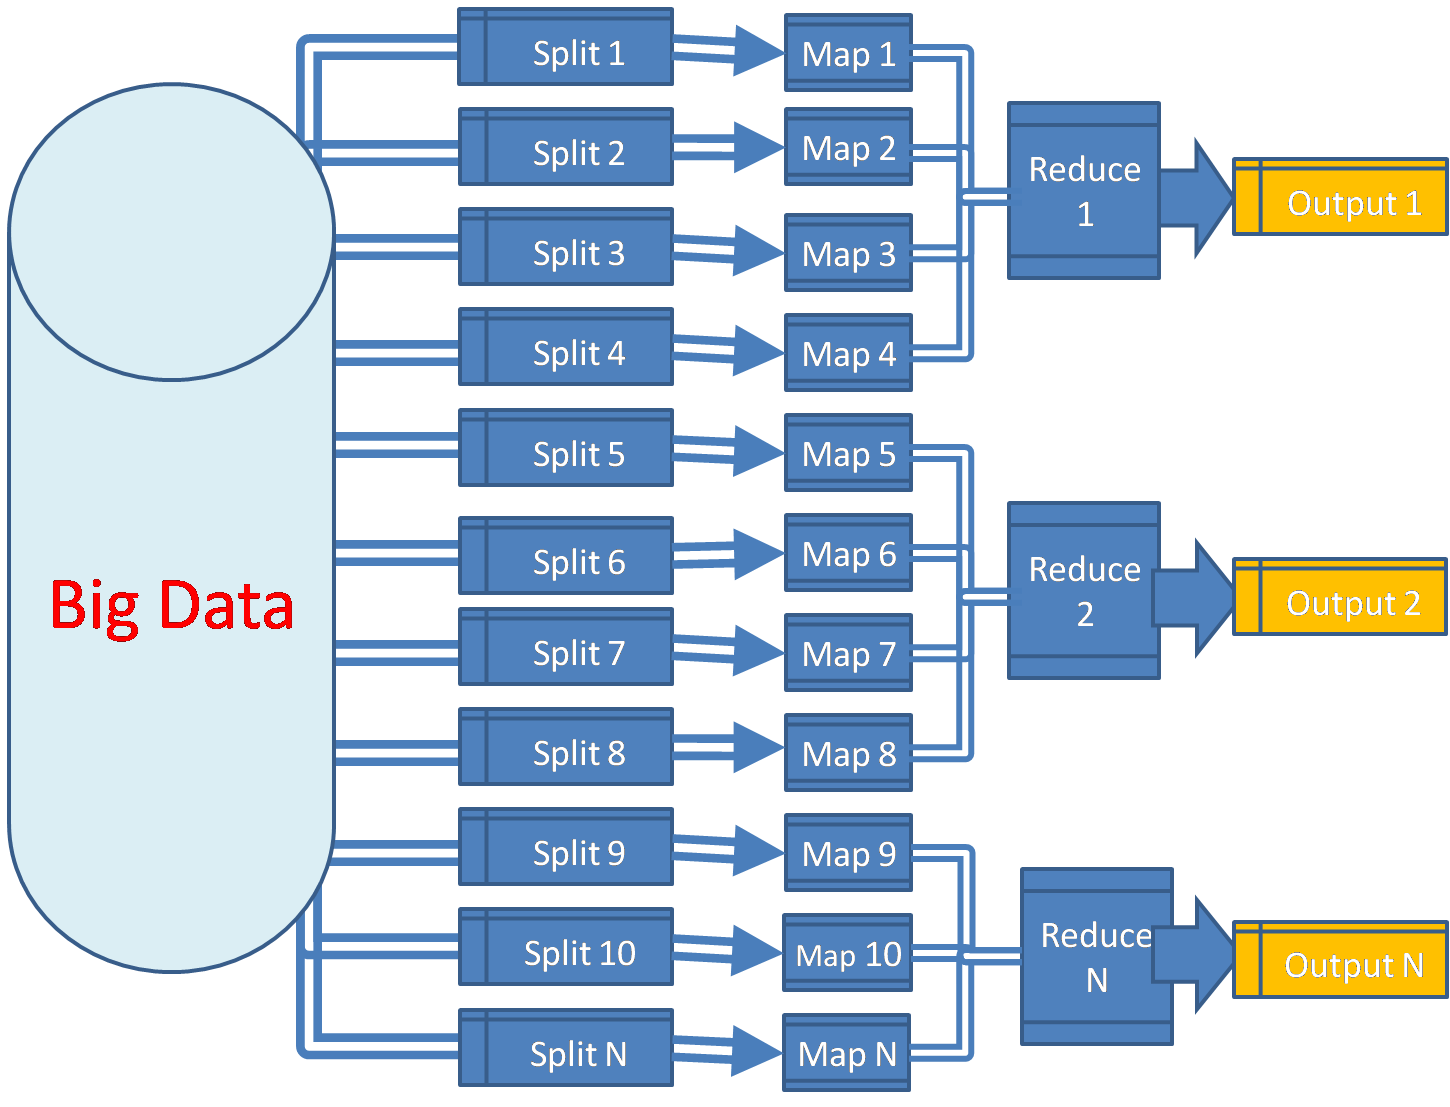
\includegraphics[scale=0.3]{map_reduce_flow.png}
	\caption{Architektura Map Reduce}
	\label{fig:@=map_reduce_schema}
\end{figure}
\subsection{Faza Shuffle w Map Reduce}
Definicja paradygmatu nic nie wspomina o fazie textit{shuffle}\footnote{tasowanie, mieszanie}. Sam paradygmat zakłada iż każdy element wychodzący z fazy map trafia do reduktora obsługującego klucz tego właśnie elementu. Oczywiście jest to przypadek idealny, który zakłada iż dane pośrednie są już posortowane bądź wszystkie elementy mają ten sam klucz (występuje jeden reduktor). W praktyce takie scenariusze nie występują często i wymagane jest zorganizowanie danych pośrednich w sposób taki by trafiły do odpowiedniego reduktora. Za tą część jest odpowiedzialna faza shuffle, która w rzeczywistości jest bardzo kosztowna gdyż sprowadza się do posortowania danych ze względu na klucz i złączenie w odpowiednie grupy na bazie klucza. Główny koszt jaki jest ponoszony to operacje wejścia-wyjścia, które są wymagane przez sortowanie i złączenie. Takie zachowanie jest widoczne na platformie Apache Hadoop.\cite{shuffle_description} Wąskie gardło paradygmatu jest ominięte w przypadku platformy Apache Spark, gdyż faza shuffle jest wykonywana w pamięci RAM co mocno redukuje koszty wejścia-wyjścia.\cite{spark_in_memory}
\newline
Praktyczna implementacja paradygmatu map reduce jest przedstawiona na rysunku \ref{fig:@=map_shuffle_reduce_schema}.\cite{map_shuffle_reduce_figure}
\begin{figure}
	\centering
	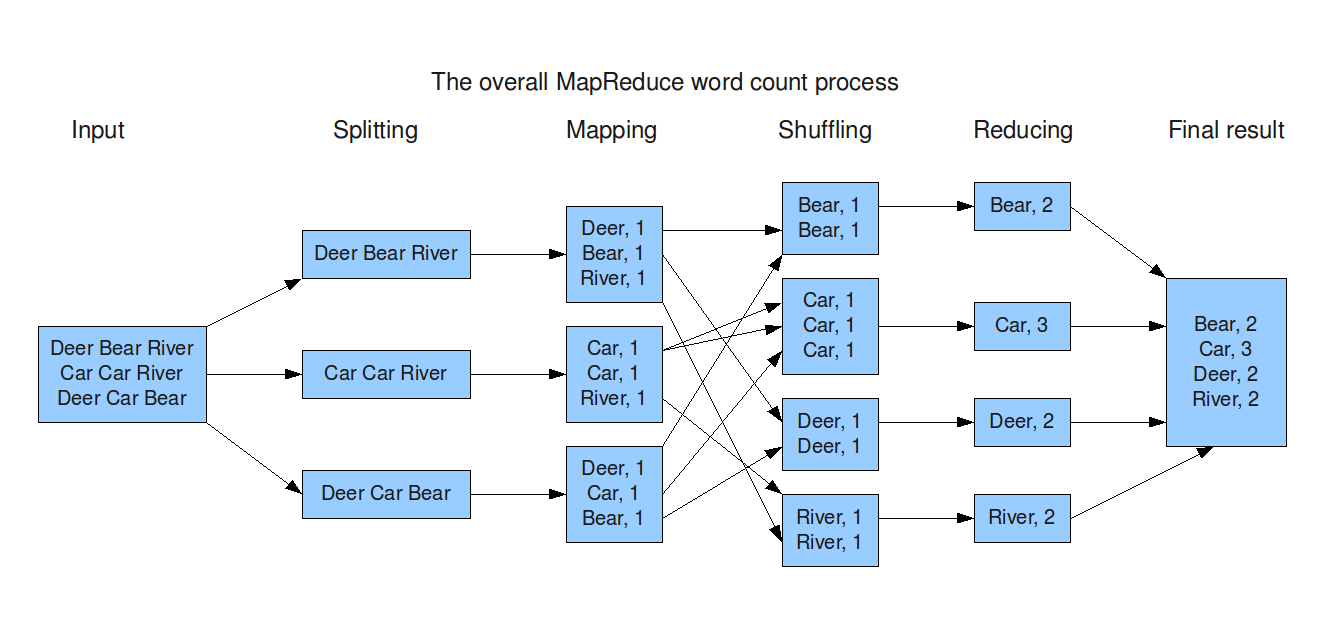
\includegraphics[scale=0.3]{MapReduceWordCount.png}
	\caption{Architektura Map Reduce wraz z fazą shuffle}
	\label{fig:@=map_shuffle_reduce_schema}
\end{figure}
\section{HDFS}
HDFS\footnote{Hadoop Distributed File System} to istotna część ekosystemów Aprache Hadoop i Apache Spark. Jest to system plików zaprojektowany specjalne do pracy w środowisku rozproszonym, którego części mogą ulegać awarii. Dzięki temu dane przechowywane w HDFS nie potrzebują kopii zapasowej, gdyż sam system z założenia dokonuje odpowiednich duplikacji. HDFS to architektura master/slave gdzie węzłem master jest jednostka o nazwie \textit{NameNode}. NameNode zawiera wszelkiego rodzaju metadane o plikach zawartych w systemie np. prawa dostępu, ilość replik. W systemie występuje jeden NameNode. Węzły slave są oznaczone nazwą \textit{DataNode} - są odpowiedzialne za przechowywanie faktycznych danych. Z racji, iż HDFS jest zaprojektowany na potrzeby danych o dużym wolumenie (od 1GB do terabajtów - dokumentacja nie definiuje konkretnej wartości) DanaNode wewnętrznie dzielą pliki na mniejsze części, które dodatkowo są duplikowane na potrzeby kopii zapasowych. HDFS jest zaimplementowany na platformie Java, także może być uruchamiany na dowolnym systemie operacyjnym. HDFS prezentuje dwa ważne założenia, które są ważne z punktu końcowego użytkownika:
\begin{itemize}
	\item Koherentność danych
	\item Przenoszenie obliczeń jest tańsze niż przenoszenie danych
\end{itemize}
Koherentność danych zapewnia łatwość w testowaniu i użytkowaniu - raz stworzony obiekt w HDFS nie zmienia swojego stanu. Jeżeli użytkownik chce zmodyfikować obiekt musi stworzyć nowy obiekt z danymi pobranymi z oryginału. Zasada przenoszenia obliczeń zapewnia zminimalizowanie transferu danych w sieci oraz poprawia ogólną przepustowość systemu.\cite{HDFS} Architektura HDFS jest przedstawiona na rysunku \ref{fig:@=hdfs_architecture}.\cite{HDFS_architecture}
\begin{figure}
	\centering
	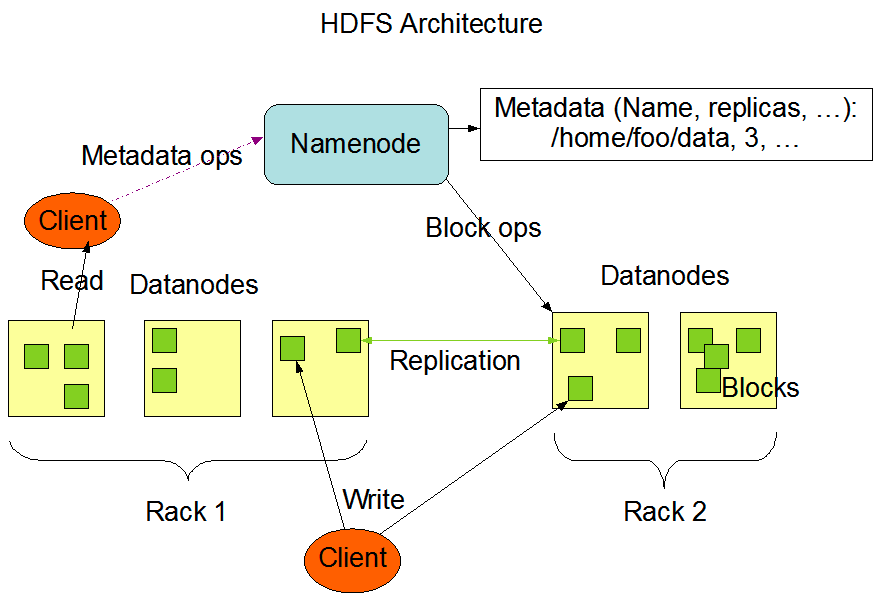
\includegraphics[scale=0.3]{hdfsarchitecture.png}
	\caption{Architektura HDFS}
	\label{fig:@=hdfs_architecture}
\end{figure}
\newline W kontekście analizy porównawczej Apache Spark i Apache Hadoop musi być zastosowany HDFS. Jest to jedyne źródło danych, na którym mogą operować obydwie platformy (Spark może pobierać dane również z innych źródeł baz typu NoSQL\footnote{Not only SQL - nierelacyjne bazy danych}).

\section{RDD}\label{rdd-section}
Platforma Spark udostępnia w swoim interfejsie programistycznym RDD\footnote{Resilient Distributed Dataset}. Jest to pojęcie, które definiuje pewien poziom abstrakcji. Można uznać, że imituje kolekcję o szczególnych właściwościach z języka Java lub Scala. Głównymi założeniami RDD są\cite{Zaharia:2012:RDD:2228298.2228301}:
\begin{itemize}
	\item Niepodzielność oraz rozproszony stan zbioru\footnote{Immutability and partitioning}
	\item Dostępność dedykowanych transformacji\footnote{Coarse-grained transformations}
	\item Odporność na błędy\footnote{Fault tolerance}
	\item Leniwa ewaluacja\footnote{Lazy evaluations}
	\item Trwałość danych\footnote{Persistence}	
\end{itemize}
\textbf{Niepodzielność zbioru danych} jest kluczowa w przypadku przetwarzania rozproszonego, gdyż zapobiega konieczności synchronizowana stanów danych. Działając na niepodzielnych jednostkach danych możemy w łatwy sposób je przetwarzać (tworzyć nowe niepodzielne zbiory danych na podstawie zbiorów wejściowych). Jednocześnie przyjmujemy, że dany zbiór danych nie znajduje się w jednej lokacji co de-facto wymusza niepodzielność i jednocześnie zapewnia łatwy interfejs programistyczny, odciążający programistę z konieczności zagłębiania się w strukturę danych. 
\newline Z racji swojej niepodzielności dostępne są \textbf{transformacje}, które są możliwe do wykonania na całym zbiorze danych równolegle np. \textit{map, filter, groupBy}. Takie podejście bardzo ułatwia zrównoleglenie operacji, jak również pozwala na rejestrację historii\footnote{lineage}. Dzięki temu w niektórych przypadkach uszkodzone dane mogą zostać odtworzone na podstawie ciągu dokonanych wcześniej operacji, zamiast być kopiowane z repliki. Takie podejście pozwala na oszczędności w postaci nośników danych. Historia jest kluczowym elementem dla \textbf{odporności na błędy} - bezpieczeństwa danych.
\newline \textbf{Leniwa ewaluacja} jest implikacją niepodzielności oraz transformacji. Użytkownik może definiować ciągi wybranych transformacji i jednocześnie kontrolować moment ich wykonania. Transformacje są leniwe co oznacza, że sama ich deklaracja nie spowoduje ich wykonania. Dopiero wywołanie akcji/operacji bądź zapisu do pamięci masowej powoduje wykonanie transformacji. Dzięki temu użytkownik może dowolnie formować dane bez konieczności interakcji z operacjami wejścia-wyjścia.
\newline \textbf{Trwałość danych} - jest to strategia, którą użytkownik może wybrać dla przechowywania RDD. Dzięki temu możliwe jest optymalizowanie przetwarzania danych bądź obliczeń w zależności od potrzeb lub możliwych zasobów.  
\begin{table}[]
	\centering
	\caption{Tabela najpopularniejszych strategi przechowywania danych dla zbioru RDD.}
	\label{RDD-strategy}
	\begin{tabular}{|l|p{6.5cm}|}
		\hline
		Strategia                             & Znaczenie                                                                                                                                                                                     \\ \hline
		Pamięć RAM                            & RDD jest przechowywane jako zdeserializowany obiekt Java, jeżeli RDD wychodzi poza dostępną pamięć  RDD jest obliczane dynamicznie za każdym odwołaniem. Strategia domyślna.                  \\ \hline
		Pamięć RAM i dysk twardy              & RDD jest przechowywane jako zdeserializowany obiekt Java, jeżeli RDD,wychodzi poza dostępną pamięć,RDD jest przechowywane na dysku twardym i stamtąd są pobierane.                            \\ \hline
		Pamięć RAM serializacja               & Działa tak samo jak strategia Pamięć RAM, lecz używa obiektów zserializowanych. Najefektywniejsza strategia jeżeli chodzi o czas wykonania obliczeń, jednocześnie wymaga wydajnego procesora. \\ \hline
		Pamięć RAM i dysk twardy serializacja & Działa tak samo jak strategia Pamięć RAM i dysk twardy, lecz używa obiektów zserializowanych.                                                                                                 \\ \hline
		Dysk twardy                           & Przechowuje RDD wyłącznie na dysku twardym.                                                                                                                                                   \\ \hline
	\end{tabular}
\end{table}
Najpopularniejsze strategie dla implementacji Java i Scala są przedstawione w tabeli \ref{RDD-strategy}. Dodatkowe strategie są opublikowane w dokumentacji Apache Spark pod adresem: \url{http://spark.apache.org/docs/latest/programming-guide.html#rdd-persistence}. Możliwości jakie oferuje RDD są o wiele większe niż te, które są dostępne w Apache Hadoop. Hadoop to czysta implementacja paradygmatu map reduce, która nie pozwala na łączenie wielu zachowań w jeden chronologiczny ciąg zdarzeń\footnote{Pipeline}. Hadoop pozwala jedynie na zrównoleglenie jednego zachowania zdefiniowanego przez użytkownika i zapisanie wyniku w pamięci masowej. Jeżeli użytkownik chce połączyć dwa lub więcej zachowań ze sobą jest zmuszony do ich zapisu i ponownego odczytu. Takie podejście zdecydowanie utrudnia implementację oraz może mieć znaczący wpływ na prędkość uzyskiwania wyników dostarczanych przez platformę. 

\section{Operacje - przypadki użycia w architekturze równoległej}
Występuje bardzo dużo zastosowań w przypadku analizy danych na platformach równoległych. Najpopularniejsze to:
\begin{itemize}
	\item Monitorowanie transakcji bankowych - selekcja tych transferów, które mogą być nielegalne dla pracownika banku
	\item Analiza plików logowania
	\item Analiza trendów rynkowych np. najpopularniejsze filmy w serwisie Netflix\footnote{www.netflix.com}
	\item Migracja danych między centrami w różnych lokalizacjach. Map zapewni transfer małych porcji danych w sieci, reduce zadba o złączenie wcześniej wysłanych danych oraz sprawdzenie czy nie uległy modyfikacji/regresji (np. poprzez sprawdzanie sumy kontrolnej). 
\end{itemize}
\chapter{Stos technologiczny} \label{chap.technology-stack}
\todo{opis aplikacji, architektura, użyte technologie, zasada działania}
\chapter{Badania}\label{chap.research}
\section{Wyniki}
Dla operacji \textit{Word Count} wyniki wydajności są przedstawione w tabeli \ref{tab:word-count-results}. Wielkość pliku wsadowego to 4 GB. Można zaobserwować, że operacja na platformie Apache Spark jest około cztery razy szybsza od Apache Hadoop. Wszystkie pomiary poza $time\_starttransfer$ oraz $time\_total$ można uznać za pomijalne dla końcowego użytkownika. Warto też odnotować iż operacja \textit{Word Count} jest najbardziej czasochłonną operacją spośród wszystkich badanych.  
\begin{table}[]
	\centering
	\caption{Wyniki wydajności dla zliczania ilości wystąpień poszczególnych fraz tekstowych (oddzielonych spacją) znalezionych w źródle danych oraz zapisu wyniku do pliku}
	\label{tab:word-count-results}
	\begin{tabular}{|l|l|l|}
		\hline
		Czas [s]    & Hadoop     & Spark      \\ \hline
		time\_namelookup    & 0.000020   & 0.000023   \\ \hline
		time\_connect       & 0.000097   & 0.000116   \\ \hline
		time\_appconnect    & 0.000000   & 0.000000   \\ \hline
		time\_pretransfer   & 0.000116   & 0.000134   \\ \hline
		time\_redirect      & 0.000000   & 0.000000   \\ \hline
		time\_starttransfer & 402.792577 & 111.232410 \\ \hline
		time\_total         & 402.792625 & 111.232446 \\ \hline
	\end{tabular}
\end{table}
\newline Dla operacji \textit{Filter} wyniki wydajności są przedstawione w tabeli \ref{tab:filter-results}. Wielkość pliku wsadowego to 4GB. Operacja \textit{Filter} jest około dwa i pół raza wolniejsza na platformie Apache Hadoop w stosunku do Apache Spark. Również w tym przypadku wszelkie pomiary poza $time\_starttransfer$ oraz $time\_total$ można uznać za pomijalne dla końcowego użytkownika. Operacja \textit{Filter} jest najkrócej trwającą, ze wszystkich badanych. 
\begin{table}[]
	\centering
	\caption{Wyniki wydajności dla zliczania ilości linii zawierających frazę tekstową zdefiniowaną przez użytkownika}
	\label{tab:filter-results}
	\begin{tabular}{|l|l|l|}
		\hline
		Czas [s]    & Hadoop    & Spark     \\ \hline
		time\_namelookup    & 0.000022  & 0.000029  \\ \hline
		time\_connect       & 0.000090  & 0.000113  \\ \hline
		time\_appconnect    & 0.000000  & 0.000000  \\ \hline
		time\_pretransfer   & 0.000110  & 0.000140  \\ \hline
		time\_redirect      & 0.000000  & 0.000000  \\ \hline
		time\_starttransfer & 42.685888 & 16.489812 \\ \hline
		time\_total         & 42.685924 & 16.489860 \\ \hline
	\end{tabular}
\end{table}
\newline Dla operacji \textit{Reject} wyniki wydajności są przedstawione w tabeli \ref{tab:reject-results}. Wielkość pliku wsadowego to 4GB. Operacja \textit{Reject} jest około pięciu razy szybsza dla platformy Apache Spark w stosunku do Apache Hadoop. Tak jak w dwóch poprzednich badanych przypadkach: \textit{Filter} oraz \textit{Word Count} pomiary poza $time\_starttransfer$ oraz $time\_total$ można uznać za pomijalne dla końcowego użytkownika.
\begin{table}[]
	\centering
	\caption{Wyniki wydajności odrzucenia linii zawierających frazę tekstową zdefiniowaną przez użytkownika oraz zapisania wyniku do pliku}
	\label{tab:reject-results}
	\begin{tabular}{|l|l|l|}
		\hline
		Czas [s]    & Hadoop     & Spark     \\ \hline
		time\_namelookup    & 0.000025   & 0.000049  \\ \hline
		time\_connect       & 0.000098   & 0.000184  \\ \hline
		time\_appconnect    & 0.000000   & 0.000000  \\ \hline
		time\_pretransfer   & 0.000118   & 0.000237  \\ \hline
		time\_redirect      & 0.000000   & 0.000000  \\ \hline
		time\_starttransfer & 238.408629 & 45.186254 \\ \hline
		time\_total         & 238.408673 & 45.186296 \\ \hline
	\end{tabular}
\end{table}

\begin{table}[]
	\centering
	\caption{Wyniki wydajności odrzucenia linii zawierających frazę tekstową zdefiniowaną przez użytkownika oraz zapisania wyniku do pliku na platformie Apache Spark ze względu na zastosowanie strategi przechowywania RDD.}
	\label{tab:reject-spark-modes-results}
	\begin{tabular}{|l|l|l|}
		\hline
		Czas{[}s{]}         & Dysk twardy & Pamięć RAM \\ \hline
		time\_namelookup    & 0.000029    & 0.000049   \\ \hline
		time\_connect       & 0.000106    & 0.000184   \\ \hline
		time\_appconnect    & 0.000000    & 0.000000   \\ \hline
		time\_pretransfer   & 0.000140    & 0.000237   \\ \hline
		time\_redirect      & 0.000000    & 0.000000   \\ \hline
		time\_starttransfer & 162.751406  & 45.186254  \\ \hline
		time\_total         & 162.751459  & 45.186296  \\ \hline
	\end{tabular}
\end{table}

\begin{table}[]
	\centering
	\caption{Wyniki wydajności dla zliczania ilości linii zawierających frazę tekstową zdefiniowaną przez użytkownika na platformie Apache Spark ze względu na zastosowanie strategi przechowywania RDD.}
	\label{tab:word-occurence-spark-modes-results}
	\begin{tabular}{|l|l|l|}
		\hline
		Czas{[}s{]}         & Dysk twardy & Pamięć RAM \\ \hline
		time\_namelookup    & 0.000021    & 0.000029   \\ \hline
		time\_connect       & 0.000096    & 0.000113   \\ \hline
		time\_appconnect    & 0.000000    & 0.000000   \\ \hline
		time\_pretransfer   & 0.000115    & 0.000140   \\ \hline
		time\_redirect      & 0.000000    & 0.000000   \\ \hline
		time\_starttransfer & 51.502827   & 16.489812 \\ \hline
		time\_total         & 51.502860   & 16.489860 \\ \hline
	\end{tabular}
\end{table}

\begin{table}[]
	\centering
	\caption{Wyniki wydajności dla zliczania ilości wystąpień poszczególnych fraz tekstowych (oddzielonych spacją) znalezionych w źródle danych oraz zapisu wyniku do pliku na platformie Apache Spark ze względu na zastosowanie strategi przechowywania RDD.}
	\label{tab:word-count-spark-modes-results}
	\begin{tabular}{|l|l|l|}
		\hline
		Czas{[}s{]}         & Dysk twardy & Pamięć RAM \\ \hline
		time\_namelookup    & 0.000023    & 0.000023   \\ \hline
		time\_connect       & 0.000099    & 0.000116   \\ \hline
		time\_appconnect    & 0.000000    & 0.000000   \\ \hline
		time\_pretransfer   & 0.000118    & 0.000134   \\ \hline
		time\_redirect      & 0.000000    & 0.000000   \\ \hline
		time\_starttransfer & 144.407036  & 111.232410 \\ \hline
		time\_total         & 144.407089  & 111.232446 \\ \hline
	\end{tabular}
\end{table}
Tabele \ref{tab:word-count-results}, \ref{tab:filter-results}, \ref{tab:reject-results} przedstawiają porównanie wszystkich badanych operacji na platformach Apache Hadoop oraz Apache Spark skonfigurowanych w sposób, który jest skalibrowany na najwyższą wydajność. W sekcji \ref{RDD-strategy} przedstawione są możliwe warianty konfiguracji platformy Apache Spark. Podczas badań zostały dokonane pomiary również w trybie wykorzystania dysku twardego do przechowywania zbioru danych RDD. Różnice w wydajności ze względu na zastosowaną strategię dla każdej badanej operacji można zaobserwować w tabelach \ref{tab:reject-spark-modes-results}, \ref{tab:word-occurence-spark-modes-results}, \ref{tab:word-count-spark-modes-results}. Wyniki zostały uzyskane na podstawie tego samego pliku wsadowego, który był wykorzystany do uzyskania wyników z tabel  \ref{tab:word-count-results}, \ref{tab:filter-results}, \ref{tab:reject-results}. Zauważalne jest, że wykorzystanie innej strategii przechowywania zbioru RDD znacząco wpływa na wydajność operacji na platformie Apache Spark. Dla operacji \textit{Reject} korzystanie ze strategii zapisu danych na dysku twardym owocuje o około 3,5 raza wolniejszym wykonywaniem. Dla operacji \textit{Filter}  zastosowanie tej samej strategii jest wolniejsze o około 3,1 raza niż strategii pamięci RAM. Operacja \textit{Word Count} traci na wydajności najmniej spośród wszystkich badanych - około 1,3 raza.  
\section{Interpretacja wyników}
Z punktu widzenia badanej wydajności wszystkie pomiary poza \textbf{time\_starttransfer} oraz \textbf{time\_total} nie są kluczowe gdyż pomijają czas pracy badanych platform. Czas całkowity jest interesujący z punktu widzenia użytkownika systemu, którego interesuje faktyczny czas uzyskania wyników. Podczas interpretacji wyników mylący może być opis przedstawiony w sekcji \ref{items:time-descriptions}. \textit{Czas przed którym pierwszy bajt danych miał zostać wysłany}. Opis ten nie dotyczy danych, które są przetwarzane na badanych platformach, lecz danych wysłanych przez odpowiedź na żądanie HTTP. Oznacza to, że dane odpowiedzi zostały wysłane po czasie, gdy wszystkie obliczenia na platformie zostały już wykonane. W związku z tym \textbf{time\_starttransfer} może zostać uznany za czas pracy przetwarzania na danej platformie.
\newline W związku z wynikami przedstawionymi w tabelach \ref{tab:filter-results}, \ref{tab:reject-results}, \ref{tab:word-count-results} możemy zaobserwować, że platforma Spark jest zdecydowanie szybsza (od dwóch i pół do pięciu razy) jeżeli chodzi o wykonywanie obliczeń i zapis wyników do pliku w systemie HDFS. Porównanie wydajności wszystkich operacji dla najbardziej wydajnej strategii przechowywania danych jest przedstawione na rysunku \ref{fig:results-comparison-bar}.
\begin{figure}[!htb]
	\centering
	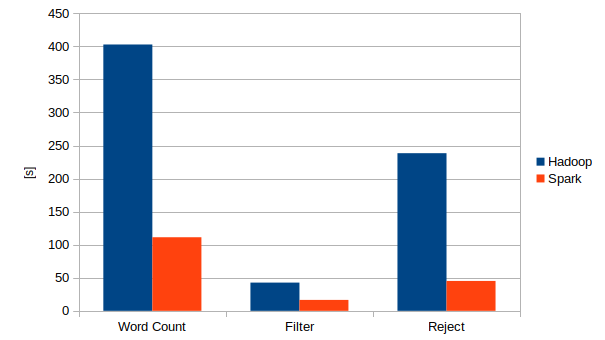
\includegraphics[scale=0.6]{results-comparison-bar.png}
	\caption{Wyniki wydajności operacji: Word Count, Filter i Reject na platformach Apache Spark oraz Apache Hadoop dla najbardziej wydajnej strategii przechowywania danych.}
	\label{fig:results-comparison-bar}
\end{figure}
Zauważalnie wyższa wydajność platformy Apache Spark wynika z zastosowania strategii przechowania danych w pamięci RAM. Dzięki dokonywaniu obliczeń w pamięci RAM uniknąć mnogości operacji wejścia oraz wyjścia co, skutkuje zauważalną różnicą w wydajności.
\begin{figure}[!htb]
	\centering
	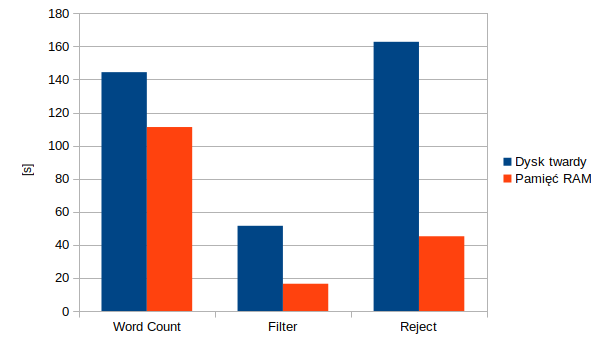
\includegraphics[scale=0.6]{results-spark-strategy-comparison-bar.png}
	\caption{Wyniki wydajności operacji: Word Count, Filter i Reject na platformie Apache Spark ze względu na zastosowaną strategię przechowywania danych.}
	\label{fig:results-spark-strategy-comparison-bar}
\end{figure}
Na rysunku \ref{fig:results-spark-strategy-comparison-bar} zostały przedstawione wyniki wszystkich operacji ze względu na zastosowaną strategię przechowywania danych w pamięci RAM lub na dysku twardym. Można zaobserwować, że wydajność operacji jest zróżnicowana w zależności od jej rodzaju. Na podstawie wykonanych badań można jednoznacznie stwierdzić, że operacje na dysku twardym będą zawsze wolniejsze od tych wykonywanych w pamięci RAM. Jednocześnie nie można ustalić jednoznacznej wartości, która pozwala wyznaczyć spadek wydajności podczas zastosowania strategii dysku twardego. Można również stwierdzić, że zastosowanie strategii dysku twardego powoduje spadek wydajności od 1,3 do 3,5 raza i jest zależne od rodzaju operacji. 
\begin{figure}[!htb]
	\centering
	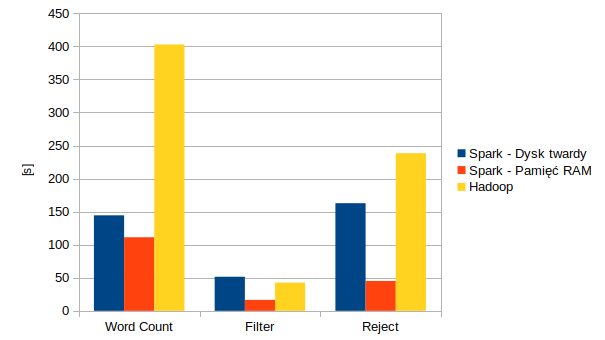
\includegraphics[scale=0.6]{results-comparison-bar-all.png}
	\caption{Wyniki zbiorcze wszystkich operacji wykonanych podczas badań.}
	\label{fig:results-comparison-bar-all}
\end{figure}
Na podstawie rysunku \ref{fig:results-comparison-bar-all} można wyciągnąć wniosek, że platforma Apache Hadoop jest najmniej wydajną spośród dwóch badanych w tej pracy magisterskiej. Niezależnie od zastosowanej operacji czas wykonywania był za każdym razem najdłuższy dla Apache Hadoop. Najbardziej wydajną platformą jest Apache Spark, który stosuje strategię przechowywania danych w pamięci RAM.    
\section{Koszty rozwoju oprogramowania i zasobów ludzkich}\label{development_human_resources}
Badane platformy Apache Spark oraz Apache Hadoop są przedstawicielami dwóch języków programowania dedykowanych na platformę JVM: Scala oraz Java. Apache Spark jest narzędziem napisanym w języku Scala i posiada interfejs programistyczny dla czterech języków programowania: Scala, Java, Python oraz R. Apache Hadoop to narzędzie oparte wyłącznie na języku Java. Rozwijanie systemów informatycznych wiąże się z wieloma aspektami takimi jak: koszty rekrutacji inżynierów posiadających wiedzę z wąskiej dziedziny np. język programowania, ramy projektowej, poszczególnych bibliotek. Innym aspektem długofalowego projektu informatycznego jest pozostawienie możliwości na rozszerzanie rozwiązania oraz integracja z innymi platformami bądź językami programowania. W przypadku Apache Hadoop rozwiązanie jest zamknięte na język Java i integracja z innymi językami programowania wymaga serializacji danych bądź też ich zapisu we wcześniej uzgodnionym formacie na przykład HDFS. W przypadku Apache Spark prace implementacji systemu mogą być prowadzone w kilku językach. Dodatkowo można wykorzystywać zaletę samego języka Scala, gdzie wszystkie biblioteki z języka Java są dostępne i nie wymagają żadnego dodatkowego nakładu pracy przy ich użyciu. W kontekście tej pracy magisterskiej zostały wykonane implementacje tych samych funkcjonalności dla dwóch języków Scala i Java. Operacja zliczenia wystąpień danej frazy w linii dla języka Scala została przedstawiona w listingu \ref{lst:scala-occurence-listing}. Ta sama operacja dla języka Java została przedstawiona w listingu \ref{lst:java-occurrence-listing}.
\begin{lstlisting}[language=scala, caption={Operacja zliczania wystąpień danej frazy w linii dla języka Scala na platformie Apache Spark},captionpos=b, label={lst:scala-occurence-listing}]
class WordOccurrence {
	def run(sparkContext: SparkContext, filePath: String, word: String) = {
	val lines: RDD[String] = sparkContext.textFile(filePath)
	val linesContainingWord = lines.filter(line => line.contains(word))
	linesContainingWord.count()
	}
}
\end{lstlisting}
\begin{lstlisting}[language=Java, caption={Operacja zliczania wystąpień danej frazy w linii dla języka Java na platformie Apache Hadoop},captionpos=b, label={lst:java-occurrence-listing}]
public class WordOccurrence {

public long run(String basePathHDFS, String wordToBeFound) throws Exception {
Path pt = new Path(basePathHDFS + "mergedTweets0.3686418061949279.txt");
Configuration conf = new Configuration();
conf.set("fs.defaultFS", basePathHDFS);
conf.set("wordToBeFound", wordToBeFound);
Job job = new Job(conf, "WordOccurrence");
job.setOutputKeyClass(Text.class);
job.setOutputValueClass(IntWritable.class);

job.setMapperClass(FilterMapper.class);
job.setReducerClass(SimpleReduce.class);

job.setInputFormatClass(TextInputFormat.class);
job.setOutputFormatClass(TextOutputFormat.class);

FileInputFormat.addInputPath(job, pt);
TimeStamp myTs = TimeStamp.getCurrentTime();
FileOutputFormat.setOutputPath(job, new Path(basePathHDFS + "hadoopWordOccurrenceResult" + myTs));
job.waitForCompletion(true);
return job.getCounters().findCounter("org.apache.hadoop.mapred.Task$Counter", "MAP_OUTPUT_RECORDS").getValue();
}

}

public class FilterMapper extends Mapper<LongWritable, Text, Text, IntWritable> {
private final IntWritable one = new IntWritable(1);
private Text word = new Text();

public void map(LongWritable key, Text value, Context context) throws IOException, InterruptedException {
String wordToBeFound = context.getConfiguration().get("wordToBeFound");
String line = value.toString();
if (line.contains(wordToBeFound)) {
context.write(word, one);
}
}
}
public class SimpleReduce extends Reducer<Text, IntWritable, Text, IntWritable> {
public void reduce(Text key, Iterable<IntWritable> values, Context context)
throws IOException, InterruptedException {
int sum = 0;
for (IntWritable val : values) {
sum += val.get();
}
context.write(key, new IntWritable(sum));
}
}
\end{lstlisting}
Nie trudno zauważyć, że ta sama funkcjonalność dla języka Scala może być przedstawiona o wiele bardziej zwięźle i czytelnie niż w języku Java. Sama różnica w ilości kodu jest zauważalna - Scala 7 linii, Java 48 linii. W przypadku utrzymywania kodu jest to bardzo ważne by rozwiązania były czytelne i łatwe do opanowania. Szczególnie istotne jest to w dużych projektach, gdzie inżynierowie często zmieniają odpowiedzialność za dany fragment funkcjonalności, bądź też występuje duża rotacja programistów. Wybór języka programowania, może też mieć znaczący wpływ na koszty rozwoju oraz utrzymania danego projektu informatycznego z racji na różnice w zarobkach ze względu na technologię. Na wykresach \ref{fig:@=salaries_contract} oraz \ref{fig:@=salaries_permanent} możemy zobaczyć koszty zatrudniania inżynierów ze względu na technologię oraz rodzaj zatrudnienia w latach 2015, 2016 oraz 2017 na terenie Wielkiej Brytanii. Dane zostały pobrane z serwisu internetowego \url{https://www.itjobswatch.co.uk}.
\begin{figure}[h]
	\centering
	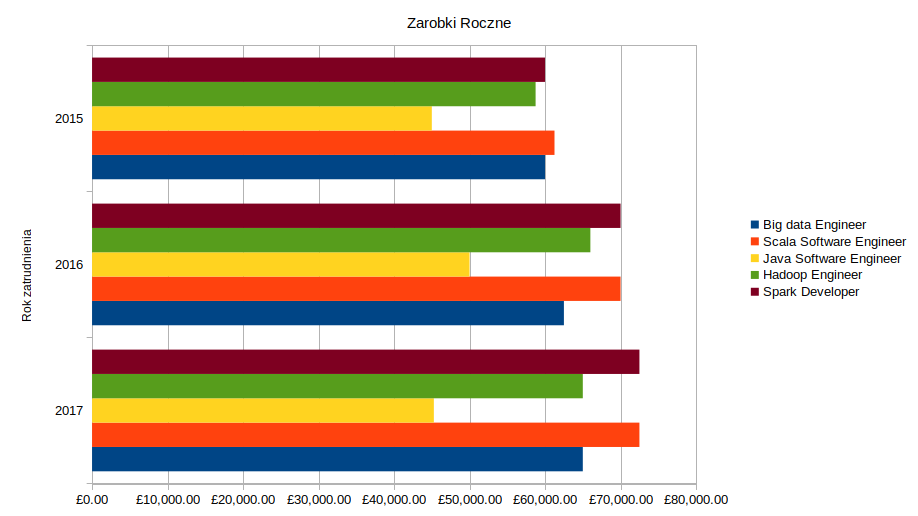
\includegraphics[scale=0.5]{salaries_contract.png}
	\caption{Trendy zarobków rocznych na terenie Wielkiej Brytanii w latach 2015, 2016 oraz 2017 dla formy zatrudnienia na kontrakt.}
	\label{fig:@=salaries_contract}
\end{figure}
\begin{figure}[h]
	\centering
	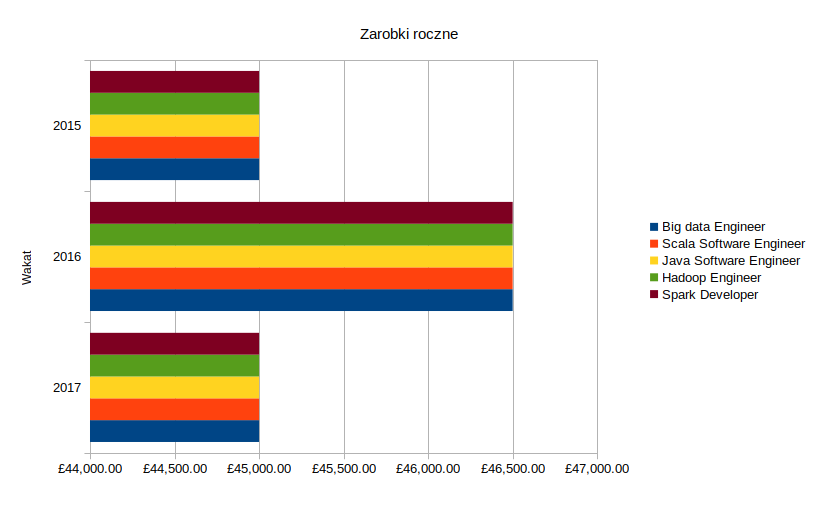
\includegraphics[scale=0.5]{salaries_permanent.png}
	\caption{Trendy zarobków rocznych na terenie Wielkiej Brytanii w latach 2015, 2016 oraz 2017 dla formy zatrudnienia stałego (umowy o pracę).}
	\label{fig:@=salaries_permanent}
\end{figure}
\newline Na podstawie rysunku \ref{fig:@=salaries_permanent} możemy zauważyć, że w kontekście rekrutacji ze względu na narzędzie bądź język programowania nie występują różnice płac dla stałej formy zatrudnienia. Jest to szczególnie istotne dla projektów o charakterystyce długofalowej oraz dużej wielkości. W przypadku formy zatrudniania stałego pracowników i dużych projektach można wybrać dowolną technologię, gdyż koszty będą relatywnie takie same (wyniki to średnie płac na dane stanowisko). Przedsiębiorstwo może również wybrać tą technologię bądź język programowania, który jest opanowany przez największą grupę docelową na rynku pracy tak by zwiększyć swoje możliwości rekrutacyjne.\newline Zupełnie odwrotnie przedstawia się sytuacja dla okresowej formy zatrudnienia tak zwany kontrakt. Dokładne dane dotyczące formy zatrudnienia na kontrakt są widoczne na rysunku \ref{fig:@=salaries_contract}. Można zaobserwować zróżnicowane płac rocznych ze względu na narzędzie bądź język programowania sięga dwudziestu siedmiu i pół tysiąca funtów rocznie. W ostatnich trzech latach najtańsze były osoby zatrudnione na kontrakt znające język programowania Java. Drugie miejsce od końca najwyższych płac rocznych zajmują inżynierowie znający Apache Hadoop. Najdroższe osoby to te posiadające kompetencje w platformie Apache Spark. 
\chapter{Podsumowanie} \label{chap.summary}
Celem tego rozdziału jest podsumowanie oraz dyskusja wyników wydajności dostarczonych przez aplikację big-data-runner. Rozdział ten stara się wskazać wyższość jednej z platform Apache Spark oraz Apache Hadoop ze względu na wymagania oraz możliwości końcowego użytkownika. Pierwsze dwa podrozdziały podsumowują wyniki testów wydajności dostarczonych przez aplikację powstałą specjalnie na potrzeby tej pracy magisterskiej. Ostatni podrozdział ocenia możliwość dalszego rozwoju powstałej aplikacji pod względem komercyjnym.   
\section{Dyskusja wyników wydajności operacji dostarczonych przez aplikację big-data-runner}
W tabelach \ref{tab:word-count-results}, \ref{tab:filter-results} oraz \ref{tab:reject-results} zostały przedstawione wyniki wydajności dla badanych operacji: \textit{Word Count}, \textit{Filter}, \textit{Reject}. Dokładny opis operacji można znaleźć w sekcji \ref{sec:user_interfaces}. Można jednoznacznie stwierdzić, że Apache Spark jest zdecydowanie szybszą platformą niż Apache Hadoop. W przypadku, gdy najważniejszym czynnikiem dla końcowego użytkownika jest prędkość analizy danych masowych, Apache Spark jest najlepszym rozwiązaniem, zapewni wyniki końcowe w krótszym czasie niż Apache Hadoop. Różnica w wydajności wynika najprawdopodobniej z architektury obydwu platform. Apache Spark korzysta domyślnie z pamięci RAM - to tam wykonywane są wszelkie obliczenia. Operacje pośrednie są kolekcjonowane w ciąg (\textit{ang. pipeline}) oraz ładowane bezpośrednio do pamięci RAM. Dzięki takiej architekturze obliczeń możliwe jest zaoszczędzenie czasu wykonywania - omijane są operacje wejścia/wyjścia. W przypadku Apache Hadoop, każda operacja pośrednia jest zapisywana na dysku, co skutkuje wolniejszym dostarczaniem wyników od dwóch i pół do pięciu razy. Dodatkową możliwością, która została wzięta pod uwagę podczas badań była strategia przechowywania zbioru RDD na platformie Apache Spark. Wyniki ze względu na strategię przechowywania zbioru RDD są przedstawione w tabelach: \ref{tab:reject-spark-modes-results}, \ref{tab:word-occurence-spark-modes-results}, \ref{tab:word-count-spark-modes-results}. Można zaobserwować spadek wydajności od 1,3 do 3,5 raza podczas zastosowania strategii dysku twardego. 
\section{Ocena obydwu platform}
Wybór między jednoznaczną wyższością spośród obydwu platform na podstawie wykonanych badań nie jest możliwy. Apache Spark i Apache Hadoop mają wiele zalet jak również wad. Niewątpliwą zaletą Apache Spark jest wydajność, która może być kluczowym aspektem dla wielu użytkowników. Dodatkowym czynnikiem przemawiającym za Apache Spark jest zwięzłość oraz czytelność kodu, która jest ważna wielu projektach informatycznych. Jest to bardzo ważny czynnik szczególnie w środowiskach korporacyjnych, gdzie rotacja osób rozwijających i utrzymujących systemy informatyczne jest częsta a każde niestandardowe, bądź mało znane rozwiązane jest uważane za wadę ze względu na trudność w skalowaniu. Jednocześnie jest narzędziem nowym, które jeszcze nie zostało opanowane przez wielu inżynierów. Może to być problematyczne w początkowej fazie dużego projektu informatycznego, gdzie wymagana jest większa liczba osób pracujących nad systemem niż w fazie utrzymania. Z racji braku wielkiej ilości osób znających Apache Spark ich wynagrodzenie rośnie w górę. Taki stosunek kosztów zatrudniania oraz rekrutacji może być czynnikiem przemawiającym za wybraniem starszej ale lepiej znanej platformy - Apache Hadoop. W przypadku rozwoju aplikacji przeznaczonej na mniejszą skalę, bądź na zamówienie klienta zewnętrznego bez zapewnienia utrzymania, warte jest rozważenie czy nie warto zastosować platformy nowszej, mniej znanej lecz zdecydowanie łatwiejszej w rozwijaniu - Apache Spark.
\section{Możliwości rozwoju komercyjnego aplikacji big-data-runner}
Aplikacja big-data-runner może być przydatnym narzędziem dla użytkowników, bądź przedsiębiorców zajmujących się przetwarzaniem danych masowych. Aplikacja jest na tyle elastyczna, że potrafi pobierać dane do testów wydajności z serwisu zewnętrznego, jak również wykonywać operacje analizy danych masowych na już wcześniej przygotowanych danych w systemie HDFS. Pod względem komercyjnym mogłaby być rozszerzona o interfejs, który umożliwiałby użytkownikowi przesyłanie jego autorskich programów wsadowych, tak by mógł dokonywać analizy danych na podstawie swoich spersonalizowanych wymagań. Dodatkową funkcją możliwą do zaimplementowania, która mogłaby być atrakcyjna dla końcowego użytkownika jest automatyczna kalkulacja kosztów najmu chmury obliczeniowej. Taka funkcjonalność dostarczyłaby użytkownikowi informację, ile kosztuje analiza danych o spersonalizowanych parametrach, zdefiniowanej wielkości oraz jaki jest koszt dostawcy sprzętu, na którym jest wdrożona aplikacja. Koszty sprzętowe oraz wyniki wydajności mogą zadecydować o wybraniu jednego z dwóch narzędzi, dostawcy sprzętu komputerowego, bądź usługodawcy chmury obliczeniowej. Takie rozszerzenie byłoby szczególnie istotne i przydatne przy ocenie opłacalności migracji z Apache Hadoop do Apache Spark. Koszty sprzętowe korzystania z Apache Spark mogą być zbliżone podczas zastosowania strategii przechowywania danych na dysku twardym. Jeżeli taka funkcjonalność dostarczałaby wartości pieniężnych co do kosztów sprzętowych, estymacja kosztów migracji z Apache Hadoop na Apache Spark jest możliwa do zrealizowana w łatwy i szybki sposób po połączeniu z danymi kosztów rekrutacji i szkoleń inżynierów. 
\nocite{Beck:2002:TDD:579193}
\nocite{Beck:2004:EPE:1076267}
\nocite{Hunt:2000:PPJ:320326}
\nocite{Martin:2008:CCH:1388398}
\bibliography{references}
\bibliographystyle{alpha}
\listoffigures
\listoftables
\end{document}
